%%-----------------Chapter 4---------------------------
\chapter{Results}
This section is broken up into the linear models which predict points, and the logistic regression which predicts whether or not a team makes the playoffs.
\section*{Multiple Linear and Ridge Regression}
\subsection*{Multiple Linear Regression}
We begin with the linear regression models. We employed two different techniques for variable selection. The first was to use AIC on the model containing every variable to reduce it. The second model was to utilize the $p$ values from the full model to create a smaller model(see Appendix G for the plots for these models). The AIC model is: \begin{center}$
	points = 11.8895(goalsPerGame) - 14.2963(goalsAgainstPerGame) + 0.1168(powerPlayPercentage) + 24.9296(winScoreFirst) + 26.3916(winOppScoreFirst) - 10.1651(winLeadSecondPer) + 24.6731(winOutshootOpp) + 23.2772(winOutshotByOpp) + 0.1465(faceOffWinPercentage) + 48.08239  
	$\end{center}
Using the AIC variable selection method to predict the 2017-2018 season generated the following values: 
	\begin{longtable}{|c|c|c|c|c|}
		\hline
		Team & Actual Points & Fit & Lower Bound & Upper Bound \\
		\hline
	ANA & 101 & 100.75284 & 99.97375 & 101.53194 \\
	ARI & 70 & 69.95098  & 68.84575 & 71.05622 \\
	BOS & 112 & 113.22077 & 112.29306 & 114.14848 \\
	BUF & 62 & 61.34851 & 60.21012 & 62.48689 \\
	CGY & 84 & 83.89612 & 83.32665 & 84.46558 \\
	CAR & 83 & 78.64918 & 77.28295 & 80.01540 \\
	CHI & 76 & 76.55805 & 75.56548 & 77.55063 \\
	COL & 95 & 92.92405 & 91.32146 & 94.52664 \\
	CBJ & 97 & 97.54118 & 96.82266 & 98.25970 \\
	DAL & 92 & 95.47584 & 94.64515 & 96.30652 \\
	DET & 73 & 70.79009 & 69.92879 & 71.65140 \\
	EDM & 78 & 78.45955 & 77.35247 & 79.56662 \\
	FLA & 96 & 92.36763 & 91.51401 & 93.22125 \\
	LAK & 98 & 103.80054 & 102.81034 & 104.79075 \\
	MIN & 101 & 100.14622 & 99.46543 & 100.82701 \\
	MON & 71 & 70.25493 & 69.04528 & 71.46458 \\
	\hline
	NAS & 117 & 112.61700 & 111.66045 & 113.57356 \\
	NJD & 97 & 94.20401 & 93.11517 & 95.29285 \\
	NYR & 80 & 77.95396 & 76.49314 & 79.41479 \\
	NYI & 77 & 77.25902 & 76.01372 & 78.50432 \\
	OTT & 67 & 68.38637 & 67.32877 & 69.44398 \\
	PHI & 98 & 95.86227 & 94.90189 & 96.82265 \\
	PIT & 100 & 100.11463 & 98.75588 & 101.47339 \\
	SJS & 100 & 99.20700 & 98.50750 & 99.90650 \\
	STL & 94 & 92.63031 & 91.82807 & 93.43255 \\
	TBL & 113 & 114.26413 & 112.97819 & 115.55006 \\
	TOR & 105 & 104.10971 & 102.95802 & 105.26140 \\
	VAN & 73 & 74.11990 & 73.02802 & 75.21179 \\
	VGK & 105 & 105.72077 & 104.52086 & 106.92069 \\
	WIN & 114 & 111.38760 & 110.38272 & 112.39248 \\
	WSH & 109 & 109.24877 & 108.09746 & 110.40008 \\
	\hline
	\end{longtable}
\captionof{table}{AIC Prediction}\label{tbl:AIC Prediction}
The $p$ value model is: \\ \begin{center}$
	points = 35.603(winScoreFirst) + 36.087(winOppScoreFirst) + 44.795(winOutshootOpp) + 42.294(winOutshotByOpp) + 12.525  
	$\end{center}
For the 2017-2018 season, the $p$ value model provided the following values:
\begin{longtable}{|c|c|c|c|c|}
	\hline
	Team & Actual Value & Fit & Lower Bound & Upper Bound \\
	\hline
	ANA & 101 &   99.39386 & 98.76494  & 100.02278 \\
	ARI & 70 &  66.88440  & 65.62004  & 68.14876 \\
	BOS & 112 &  112.15517 & 111.09914 & 113.21120 \\ 
	BUF & 62 &  61.61019  & 60.34175  & 62.87862 \\
	CGY & 84 & 86.50087 & 85.89007 & 87.11167 \\
	CAR & 83 & 76.55718 & 75.21138 & 77.90297 \\
	CHI & 76 &  74.48080 & 73.50540 & 75.45621 \\
	COL & 95 &   91.48654 & 90.27831 & 92.69478 \\
	CBJ & 97 &  99.37009 & 98.56669 & 100.17348 \\
	DAL & 92 & 95.55320 & 94.54216 & 96.56423 \\
	DET & 73 & 68.86493 & 67.86799 & 69.86188 \\
	EDM & 78 & 81.65953 & 80.83764 & 82.48141 \\
	FLA & 96 & 94.57227 & 93.80385 & 95.34068 \\
	LAK & 98 & 102.03421 & 100.72097 & 103.34744 \\
	MIN & 101 & 100.17189 & 99.49410 & 100.84968 \\
	MON & 71 & 69.64649 & 68.37613 & 70.91685 \\
	NAS & 117 & 110.43911 & 109.43556 & 111.44266 \\
	NJD & 97 & 97.26480 & 96.42495 & 98.10466 \\
	NYR & 80 & 79.71466 & 78.88915 & 80.54018 \\
	NYI & 77 & 79.78500 & 78.96401 & 80.60599 \\
	OTT & 67 & 70.26269 & 69.18237 & 71.34301 \\
	\hline
	PHI & 98 & 94.04029 & 93.18841 & 94.89217 \\
	PIT & 100 & 101.05045 & 100.16146 & 101.93943 \\
	SJS & 100 & 99.11771 & 98.37639 & 99.85902 \\
	STL & 94 & 94.61598 & 93.76003 & 95.47192 \\
	TBL & 113 & 116.02619 & 114.91506 & 117.13731 \\
	TOR & 105 & 101.56422 & 100.61952 & 102.50893 \\
	VAN & 73 & 72.16710 & 70.95580 & 73.37839 \\
	VGK & 105 & 110.72874 & 109.69436 & 111.76313 \\
	WIN & 114 & 110.03455 & 109.12397 & 110.94514 \\
	WSH & 109 & 109.70151 & 108.43704 & 110.96598 \\
	\hline
\end{longtable}
\captionof{table}{$p$ value Prediction}\label{tbl:$p$ value Prediction}
Now that we have our predictions, we compare them to the actual points. Below are box plots for each model's error (see Appendix E for a table of error values;
see figure 4.1 for the AIC prediction error; 4.2 for the $p$ value error). \\
\begin{figure}
	\centering
	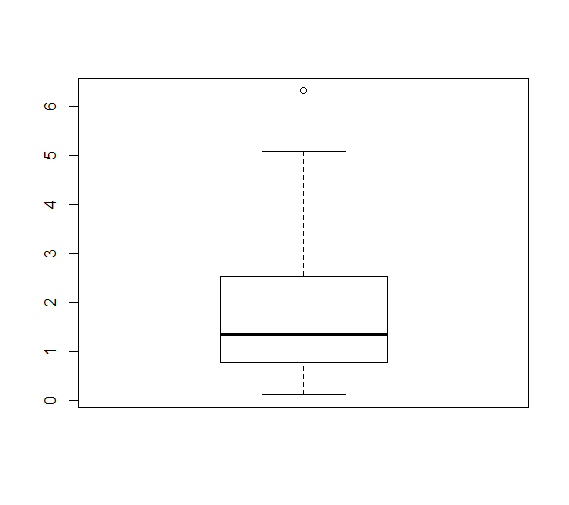
\includegraphics[width=0.7\linewidth]{AICPredictionError}
	\caption{AIC Error Plot}
	\label{fig:aicpredictionerror}
\end{figure}
\begin{figure}
	\centering
	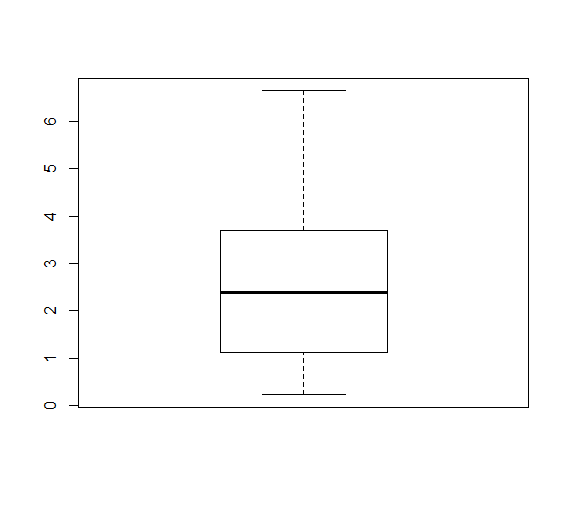
\includegraphics[width=0.7\linewidth]{pvalueerror}
	\caption{P Value Error}
	\label{fig:pvalueerror}
\end{figure}
\newpage
We now look at the model plots for the two methods; (see Appendix G for the plots). For the AIC models residual versus fitted value plot we can see that a linear relationship is a reasonable assumption, and that there are two outliers. For the normal $q-q$ plot, we can see that most of the points are on the line, so normality is assumed. The scale-location plot tells us that a linear relationship is a reasonable assumption. The residual versus leverage plot shows no Cook's Distance anywhere; therefore, everything was approximated well, with no significantly influential points. The p value residual versus fitted value plot shows us that a linear relationship is a reasonable assumption, but we have 3 outliers. The normal $q-q$ plot tells us that normality is assumed. The scale-location plot shows us that a linear relationship is an reasonable assumption. However, the residual versus leverage plot tells us that we have an influential point. 
The majority of the predictions made using the AIC model were one to two points off the actual value. The most extreme error occurred in the case of the Los Angeles Kings: the prediction was five points off what the team actually achieved. One reason for this is that LA had the lowest goals against per game in the NHL during this season at $2.890$ goals against. In the model we have $- 14.2963$$(goalsAgainstPerGame)$, which would have less weight for Los Angeles thus raising the predicted value. Another reason is that LA was ninth in wins when the opponent scored first at 0.4 or 40\%, which is another variable with a heavy weight in our prediction function. The second most extreme error was in the case of the Nashville Predators. The prediction was four points off the actual value; one reason for this is that, similar to LA, the Predators were second in goals against per game at 2.488. Other statistics of LA lend to the conclusion that good defensive teams, that limit their goals against, tend to have more points. According to this model. LA was 16th in goals per game; 18th in power play percentage; 7th in wins when the team scored first; 9th when the opponent scored first; 11th in wins when leading after the second period; 7th in wins when out shooting the opponent; 21st in wins when out shot and finally 17th in face off win percentage. For the p value model, most estimates were off significantly; up to almost 4 points. This is really due to the model lacking no deduction for poor defensive play (i.e. $- 14.2963(goalsAgainstPerGame)$ and $- 10.1651(winLeadSecondPer)$). The model also rewards teams for having lots of shots. For example, the Boston Bruins were first in wins when the opponent scored first, and third in wins when you have more shots then your opponent. This increased the value of their prediction. Therefore, this model is a better exploratory model then a predictor model. This model can be used to explore the effect of scoring and shooting more frequently on overall points. The next step is to talk about the ridge regression models.
\subsection*{Ridge Regression}
For the ridge regression model R calculated 99 different $k$ values(or $\lambda$ as R calls it) and fit all 24 variables to it. This created the ridge trace below.
\newpage
\begin{figure}
	\centering
	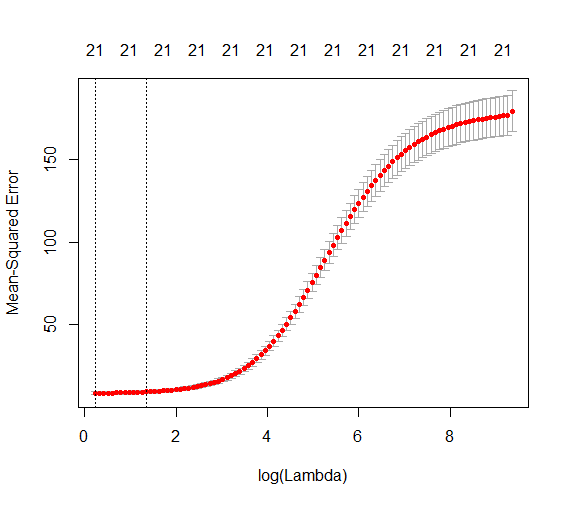
\includegraphics[width=0.7\linewidth]{RidgeTrace}
	\caption{Ridge Trace}
	\label{fig:ridgetrace}
\end{figure}
\newpage
This method had the predictions: \newpage
\begin{longtable}{|c|c|c|}
	\hline
	Team & Actual Value & Points \\
	\hline
ANA & 101 & 99.06189 \\
ARI & 70 & 71.28012 \\
BOS & 112 & 112.35062 \\
BUF & 62 &  63.93565 \\
CGY & 84 &  84.82366 \\
CAR & 83 &  79.65816 \\
CHI & 76 &  77.87249 \\
COL & 95 &  94.57622 \\
CBJ & 97 & 96.59796 \\
DAL & 92 & 95.01542 \\
DET & 73 & 72.94090 \\
EDM & 78 & 80.39590 \\
FLA & 96 & 93.44379 \\
LAK & 98 & 103.62926 \\
MIN & 101& 99.55909 \\
MON & 71 & 72.73987 \\
NAS & 117 & 110.75469 \\
NJD & 97 & 94.49269 \\
NYR & 80 & 80.68079 \\
NYI & 77 & 80.14972 \\
OTT & 67& 70.15000 \\
\hline
PHI & 98 & 95.42240 \\
PIT & 100 & 99.72449 \\
SJS & 100 & 99.38607 \\
STL & 94 & 93.23966 \\
TBL & 113 & 112.73388 \\
TOR & 105 & 104.18809 \\
VAN & 73 & 76.84935 \\
VGK & 105 & 105.25785 \\
WIN & 114 &111.00241 \\
WSH & 109 &106.87331 \\
	\hline
\end{longtable}
\captionof{table}{Ridge Regression Prediction}\label{tbl:Ridge Regression Prediction}
Next we need to compare the predictions to the actual points. Below this are box plots for the model error (see Appendix E for a table of error values).
\begin{figure}
	\centering
	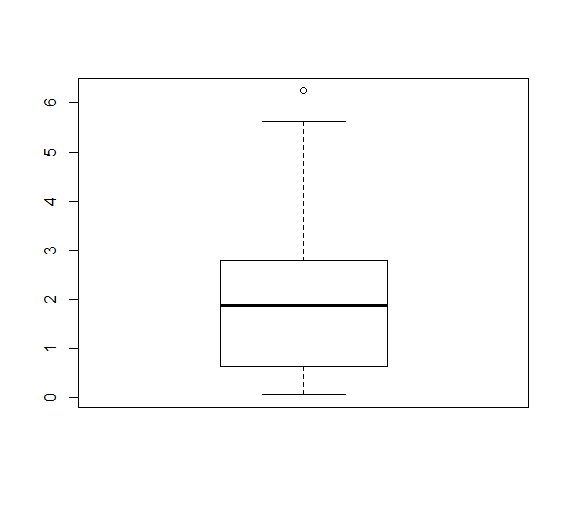
\includegraphics[width=0.7\linewidth]{RidgePredictionError}
	\caption{Ridge Prediction Error}
	\label{fig:ridgepredictionerror}
\end{figure}\newpage
The most extreme error in this model is for the Nashville Predators, 6 points off the actual point value. Since the ridge regression model takes every variable in our data set, the error is largely due to them being in the top 15 for almost every variable in our set. The ridge regression model weighs every statistic evenly. The next step is to talk about our logistic regression model.
\section*{Logistic Regression}
For the logistic regression models, we are predicting the probability that a team makes the playoffs. For this model we use every variable, rather than using AIC. The reason for this is AIC would default to the model containing just the intercept every single time, regardless of whether we use forward selection, backward selection or stepwise selection. Therefore our model is:\begin{center}$
	madePlayoffs = -596.2016 + 0.6785186(pts) + 17.31825(goalsPerGame) - 6.797520(goalsAgainstPerGame) - 18.07236(evGAARatio) - 0.1268944(powerPlayPercentage) - 0.03467402(powerPlayGoals) - 0.1270233(powerPlayGoalsAgainst) - 0.004215109(powerPlayOpportunities) - 0.04239098(penaltyKillPercentage) - 0.3554432(shotsPerGame) - 16.05426(winLeadFirstPer) + 3.368749(winLeadSecondPer) + 3.367920(winOutshootOpp) + 12.48498(winOutshotByOpp) + 0.07043268(faceOffsTaken) - 0.1464181(faceOffsWon) + 7.594018(faceOffWinPercentage) - 1.656188(shootingPctg) + 214.9347(savePctg)   
	$\end{center}
Below is the table of probabilities that a team makes the playoffs: \newpage
\begin{longtable}{|c|c|}
	\hline
	Team & Probabilities \\
	\hline
ANA* & 9.999420e-01 \\
ARI & 1.371664e-10 \\
BOS* & 1.000000e+00 \\
BUF & 8.768418e-13 \\
CGY & 3.308281e-04 \\
CAR & 3.893547e-04 \\
CHI & 6.972501e-07 \\
COL* & 4.071688e-01 \\
CBJ* & 9.659823e-01 \\
DAL & 8.537965e-01 \\
DET & 5.600266e-09 \\
EDM & 5.735255e-07 \\
FLA & 7.984136e-01 \\
LAK* & 9.981411e-01 \\
MIN* & 9.990949e-01 \\
MON & 1.113290e-10 \\
NAS* & 1.000000e+00 \\
NJD* & 9.873069e-01 \\
NYR & 4.818513e-06 \\
NYI & 4.298577e-06 \\
OTT & 3.435248e-12 \\
\hline
PHI* & 9.995894e-01 \\
PIT* & 9.995588e-01 \\
SJS* & 9.989304e-01 \\
STL & 5.896700e-01 \\
TBL* & 1.000000e+00 \\
TOR* & 9.999801e-01 \\
VAN & 3.011319e-10 \\
VGK* & 9.997866e-01 \\
WIN* & 1.000000e+00 \\
WSH* & 1.000000e+00 \\
	\hline
\end{longtable}
Here * indicates if a team made the playoffs. This model has Anaheim, Boston, Vegas, Winnipeg, Washington, Toronto, Tampa Bay, San Jose, Philadelphia , Pittsburgh, New Jersey, Nashville, Minnesota, LA, Columbus and Dallas all having a high probability of making the playoffs. The only team out of this list that did not make the playoffs during this season was Dallas, (instead, Colorado made it). One possible reason for this is that during the 2013-2014 season the NHL changed the playoff format; rather than the top 8 teams from each conference making it; the top 3 teams from each division made it and the two final teams representing each conference were wild card teams. No good packages were available to create the model plots for logistic regression. Now we go on to the conclusion.